\section{Methodology}
\label{sec:methodology}

\begin{figure*}[t!]
    \centering
    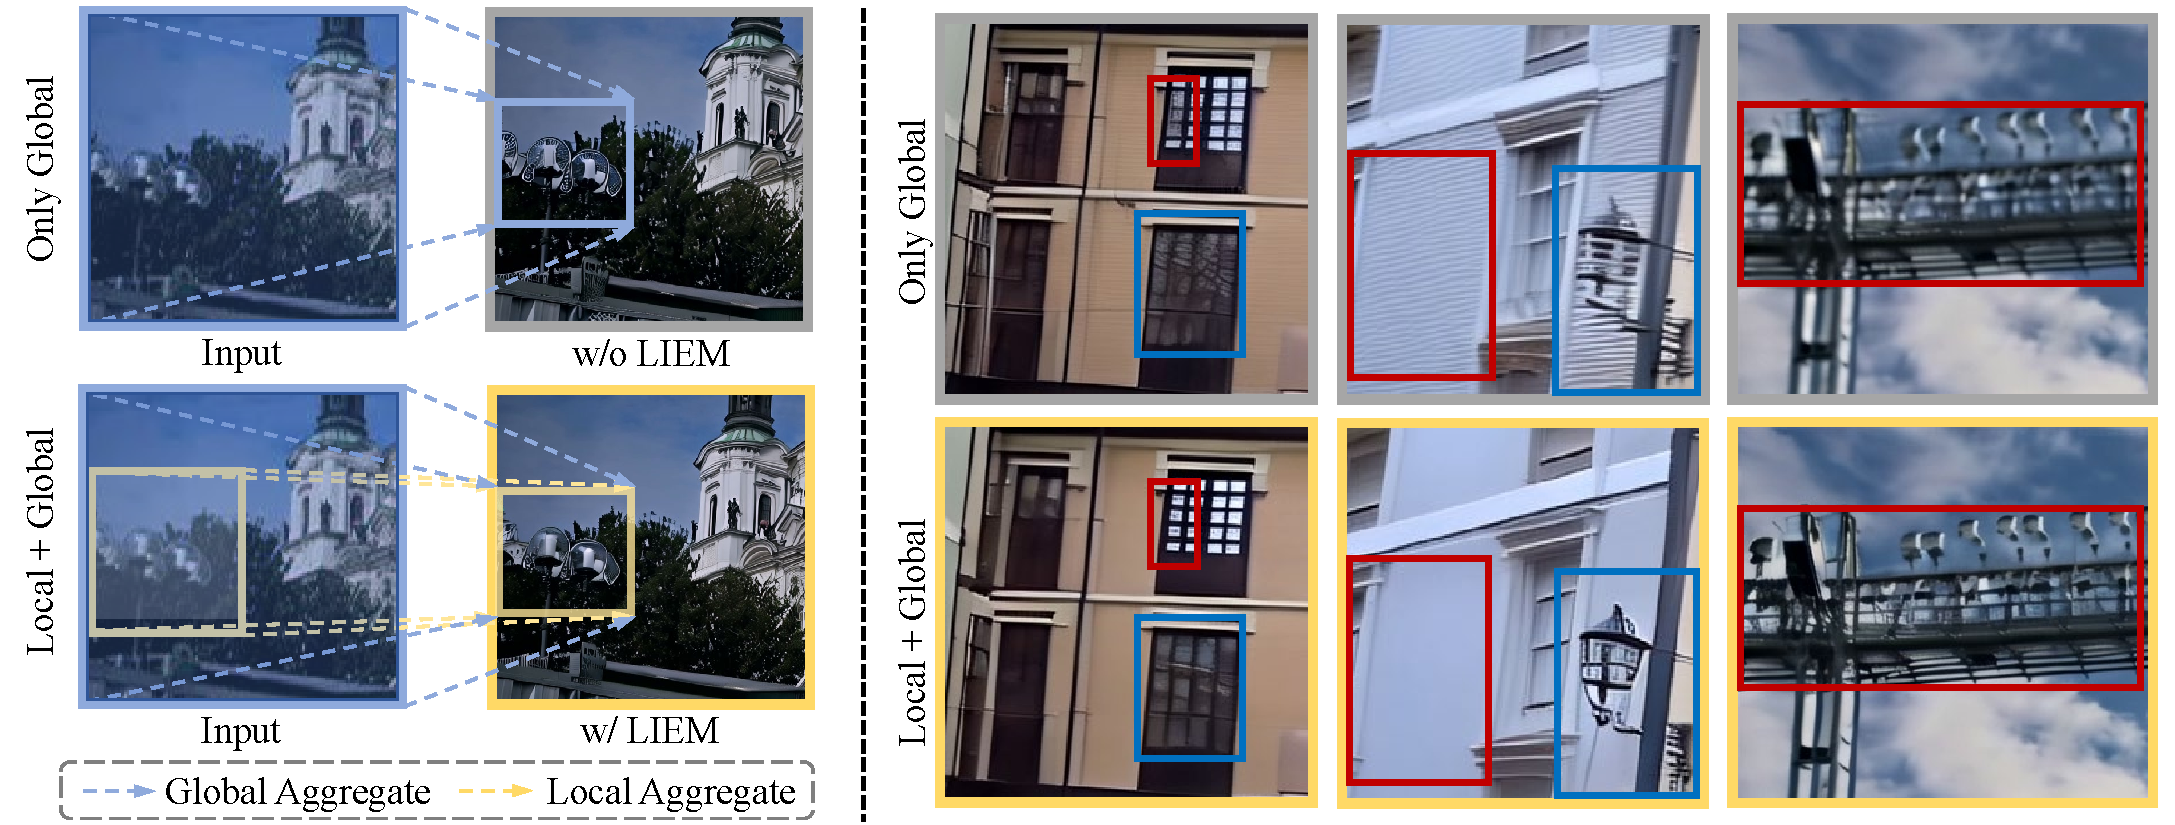
\includegraphics[width=0.98\linewidth]{figure/liem_motivation.pdf}\vspace{-2mm}
    \caption{\textbf{Motivation of LIEM.} \textbf{Left:} schematic diagram illustrating the impact of using only global structure versus a combination of local and global structures. \textbf{Right:} visual comparison on real-world and synthetic videos. (\textbf{Zoom-in for best view})}
    \label{motivation:liem}
\end{figure*}

\begin{figure*}[t!]
    \centering
    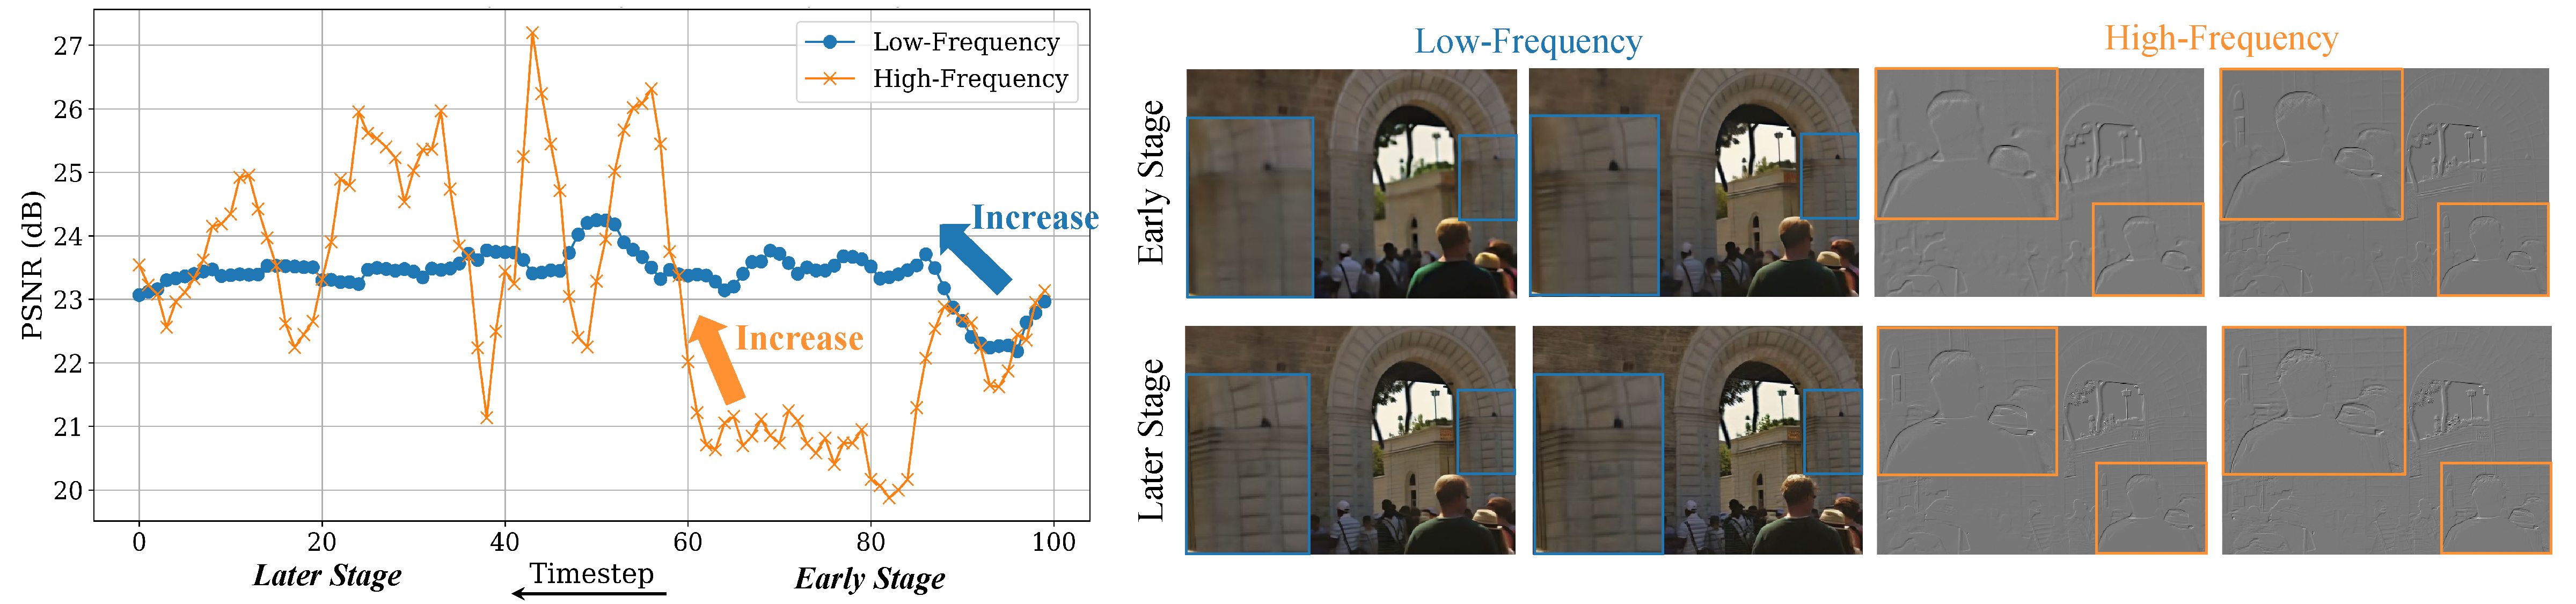
\includegraphics[width=1\linewidth]{figure/daf_motivation.pdf}
    \caption{\textbf{Motivation of DF Loss.} \textbf{Left}: PSNR curves of low- and high-frequency components relative to ground truth across diffusion steps. The low-frequency PSNR increases during the early diffusion steps, while the high-frequency PSNR rises in the later diffusion steps. 
    \textbf{Right}: visual results of low- and high-frequency components at different diffusion stage. (\textbf{Zoom-in for best view})}
    \label{motivation:daf}
\end{figure*}

\subsection{Overview}
\label{subsec:overview}

\paragraph{Modules.}
% \textbf{Modules.}
The~\name~primarily includes four modules: VAE \cite{kingma2013auto}, text encoder \cite{radford2021learning, raffel2020exploring}, ControlNet \cite{zhang2023adding} and T2V model \cite{zhang2023i2vgen, yang2024cogvideox} with Local Information Enhancement Module (\textbf{LIEM}) to alleviate the artifacts (further analysis is provided in Sec.~\ref{subsec:LIEM}). 
As depicted in Figure~\ref{fig:overview}, the VAE encoder takes HR videos $X_H$ and LR videos $X_L$ as input to generate latent tensors $Z_H$ and $Z_L$, respectively. The text encoder is responsible for generating text embeddings $c_{text}$ to provide high-level information. ControlNet takes $Z_L$ and $c_{text}$ as input to guide the T2V model output. Finally, the T2V model $\phi_\theta$ with \textbf{LIEM} receives noisy input $Z_t = \alpha_t Z_H + \sigma_t \epsilon$ ($t$ denotes diffusion step, $\alpha_t$ and $\sigma_t$ are noise scheduler parameters), $c_{text}$ and the control signal from ControlNet $c_{l}$ to predict the velocity $v_t \equiv \alpha_t \epsilon - \sigma_t Z_H$ \cite{salimans2022progressive}. 

\vspace{-1em}
\paragraph{Losses.}
% \noindent
% \textbf{Losses.}
We utilize v-prediction objective in optimization:
\begin{equation}
    \mathcal{L}_{v} = \mathbb{E}[\| v_t - \phi_\theta(Z_t, c_{text}, c_{l}, t) \|_2^2].
\end{equation}
%Due to the strong generalization ability of T2V models, using only the v-prediction objective for optimization may result in restored outputs with low fidelity, which is critical for video super-resolution tasks. To address this issue, we propose Dynamic Frequency (\textbf{DF}) Loss, which dynamically adjusts the constraint degree on the high-frequency and low-frequency components of the predicted $\hat{X}_H$ across different diffusion steps. The overall optimization objective for~\name~is as follows:
%
Given the strong generalization ability of T2V models, relying solely on the v-prediction objective for optimization may lead to restored outputs with low fidelity, an essential factor in video super-resolution tasks. 
To address this, we introduce Dynamic Frequency (\textbf{DF}) Loss, which adaptively adjusts the constraint on high- and low-frequency components of the predicted $\hat{X}_H$ across different diffusion steps. 
The overall optimization objective for~\name~is as follows:
%
\begin{equation}
    \mathcal{L}_{total} = \mathcal{L}_{v} + b(t)\mathcal{L}_{DF}(\hat{X}_H, X_H),
\end{equation}
where $b(t)= 1 - \frac{t}{t_{max}}$ is a weighting function ($t_{max}$ is set to 999) to balance $\mathcal{L}_{v}$ and $\mathcal{L}_{DF}$. 
With the proposed LIEM and DF loss,~\name~achieves high spatio-temporal quality, reduced artifacts and enhanced fidelity.

\subsection{Local Information Enhancement Module}
\label{subsec:LIEM}

\paragraph{Motivation.} 
% \noindent
% \textbf{Motivation.}
%Most T2V models primarily employ global attention mechanism \cite{liu2021global}, which is well-suited for the text-to-video task. This design choice aligns with the need to generate entire videos from scratch, capturing the global information. However, this approach may not be optimal for real-world video super-resolution, where complex degradations exist and local details are also important \cite{kong2022residuallocalfeaturenetwork}.
%
Most T2V models primarily use a global attention mechanism~\cite{liu2021global}, which is well-suited to text-to-video tasks by capturing global information to generate complete videos from scratch. 
However, this approach may be suboptimal for real-world video super-resolution, where complex degradations occur and local details are crucial~\cite{kong2022residual}.
%
Relying solely on global attention mechanisms presents two drawbacks for real-world video super-resolution: 
$1$) It \textit{complicates degradation removal}, as it processes the entire degraded video at once (the first and second columns in Figure~\ref{motivation:liem} (right)).
$2$) It \textit{lacks local details}, resulting in blurry outputs (the third column in Figure~\ref{motivation:liem} (right)). 

%As shown in Figure~\ref{motivation:liem}, when only using global attention mechanisms, there are two disadvantages for real-world video super-resolution: 1) It increases the difficulty of removing degradations since it handles the entire degraded video (\textit{e.g.,} see the first and second column of Fig. \ref{motivation:liem} (right)). 2) It lacks local information, leading to blurry results (\textit{e.g.,} see the third column of Figure~\ref{motivation:liem} (right)). 

\vspace{-1em}
\paragraph{Details of LIEM.}
% \noindent
% \textbf{Details of LIEM.}
To address the above issues, we propose a simple but effective approach: adding a \textit{Local Information Enhancement Module} (LIEM) before the global attention block to make T2V model pay more attention to local information. It can be expressed by:
% To address these issues, we propose a simple yet effective approach that integrates a LIEM before the global attention block to encourage the T2V model to better capture local details: %. This can be expressed as:
\begin{equation}
    L(F_I) = Sigmoid(Conv_{3\times3}(Concat(AP(F_I), MP(F_I)))),
\end{equation}
\begin{equation}
    F_O = G(L(F_I) \cdot F_I) + F_I,
\end{equation}
where $AP(\cdot)$ and $MP(\cdot)$ denote average pooling and max pooling, respectively. $F_I$ and $F_O$ represent the input and output features, while $G(\cdot)$ and $L(\cdot)$ refer to the global attention block and LIEM. We adopt the local attention block in CBAM \cite{woo2018cbam} as LIEM for simplicity. 
Additional analysis on the impact of adding LIEM is provided in Sec.~\ref{sec:liem_ablation}.
%
%where $AP(\cdot)$ and $MP(\cdot)$ denote average pooling and max pooling, respectively. $F_I$ and $F_O$ represent the input and output features, while $G(\cdot)$ and $L(\cdot)$ refer to the global attention block and LIEM. As the design of LIEM is not central to our~\name~ approach, we adopt the local attention block from CBAM \cite{woo2018cbam} for simplicity. Additional analysis on the impact of LIEM is provided in
%
Intuitively, as shown in the second row of Figure~\ref{motivation:liem} (left), %with LIEM, the T2V model can first deal with local region degradation and then aggregate global features, reducing the difficulty of degradation removal and alleviating generated artifacts. 
incorporating LIEM enables the T2V model to address local region degradation first and then aggregate global features. 
This approach reduces the complexity of degradation removal and mitigates artifacts. 
Furthermore, the T2V model with LIEM produces clearer, more detailed results due to the enriched local information.
 
\subsection{Dynamic Frequency Loss}
\label{subsec:daf}


\begin{table*}[t!]
    \caption{Quantitative evaluations on diverse VSR benchmarks from synthetic (UDM10, REDS30, OpenVid30) and real-world (VideoLQ) sources. The best performance is highlighted in \textbf{bold}, and the second-best in \underline{underlined}. E$^*_{warp}$ refers to E$_{warp}$ ($\times10^{-3}$).} \label{tab:my_label}
    \centering
    \resizebox{\textwidth}{!}{
    \begin{tabular}{cc|cccc|cccccc}
    \hline
    \multirow{2}{*}{Datasets} & \multirow{2}{*}{Metrics} & Real-ESRGAN & DBVSR & RealBasicVSR & RealViformer & ResShift & StableSR & Upscale-A-Video & MGLDVSR & Ours \\ 
    ~ & ~ & ICCVW 2021 & ICCV 2021 & CVPR 2022 & ECCV 2024 & NeurIPS 2023 & IJCV 2024 & CVPR 2024 & ECCV 2024 & - \\ \hline \hline
    \multirow{5}{*}{UDM10} & PSNR$\uparrow$ & 22.41 & 19.65 & 23.64 & \textbf{24.00} & 22.90 & 23.50 & 21.29 & 23.74 & \underline{23.91} \\
    ~ & SSIM$\uparrow$ & 0.6476 & 0.4747 & 0.6842 & \underline{0.6896} & 0.5451 & 0.6599 & 0.5967 & 0.6826 & \textbf{0.7164} \\
    ~ & LPIPS$\downarrow$ & 0.2769 & 0.4566 & 0.2514 & 0.2325 & 0.4036 & 0.2785 & 0.3006 & \underline{0.2195} & \textbf{0.1885} \\
    ~ & DOVER$\uparrow$ & 0.4831 & 0.0959 & 0.5039 & 0.5055 & 0.3252 & 0.3490 & \underline{0.5309} & 0.4896 & \textbf{0.5422} \\
    ~ & E$^*_{warp}$ $\downarrow$ & 11.17 & 12.56 & 5.14 & 3.57 & 12.69 & 8.89 & \underline{2.83} & 6.03 & \textbf{2.68} \\ \hline
    \multirow{5}{*}{REDS30} & PSNR$\uparrow$ & 19.56 & 14.85 & \underline{20.85} & \textbf{20.86} & 19.93 & 20.32 & 19.71 & 20.57 & 20.29 \\
    ~ & SSIM$\uparrow$ & 0.4862 & 0.2941 & \textbf{0.5469} & 0.5377 & 0.4261 & 0.5043 & 0.4315 & 0.5113 & \underline{0.5411} \\
    ~ & LPIPS$\downarrow$ & 0.3376 & 0.5915 & 0.2899 & \underline{0.2597} & 0.4422 & 0.3857 & 0.3443 & \textbf{0.2240} & 0.2804 \\
    ~ & DOVER$\uparrow$ & 0.3182 & 0.0600 & 0.3483 & 0.3400 & 0.2221 & 0.2519 & 0.2857 & \underline{0.3857} & \textbf{0.4017} \\
    ~ & E$^*_{warp}$ $\downarrow$ & 19.1 & 18.00 & 8.32 & \textbf{6.06} & 17.40 & 22.14 & 15.65 & 12.28 & \underline{7.30} \\ \hline
    \multirow{5}{*}{OpenVid30} & PSNR$\uparrow$ & 24.62 & 21.14 & 24.63 & \textbf{26.21} & 24.29 & 24.91 & 24.41 & 24.73 & \underline{25.30} \\
    ~ & SSIM$\uparrow$ & 0.7778 & 0.5887 & 0.7759 & \underline{0.8080} & 0.6070 & 0.7633 & 0.7167 & 0.7686 & \textbf{0.8371} \\
    ~ & LPIPS$\downarrow$ & 0.1994 & 0.4207 & 0.2297 & \underline{0.1881} & 0.3902 & 0.2102 & 0.2479 & 0.2074 & \textbf{0.1011} \\
    ~ & DOVER$\uparrow$ & 0.6992 & 0.1819 & \underline{0.7345} & 0.7275 & 0.5435 & 0.6368 & 0.7201 & 0.7191 & \textbf{0.7393} \\
    ~ & E$^*_{warp}$ $\downarrow$ & 8.46 & 12.11 & 4.12 & \underline{2.52} & 9.78 & 8.87 & 4.72 & 4.82 & \textbf{1.82} \\ \hline \hline
    \multirow{4}{*}{VideoLQ} & ILNIQE$\downarrow$ & 27.95 & 27.19 & 26.29 & 26.11 & 25.92 & 29.97 & \underline{24.49} & \textbf{23.94} & 25.35 \\
    ~ & DOVER$\uparrow$ & 0.4967 & 0.3392 & \underline{0.5285} & 0.4804 & 0.4113 & 0.4775 & 0.4833 & 0.5319 & \textbf{0.5431} \\
    ~ & E$^*_{warp}$ $\downarrow$ & 8.00 & 7.75 & 6.52 & \textbf{5.10} & 8.33 & 9.26 & 10.89 & 7.82 & \underline{6.38} \\ \hline
    \end{tabular}}
\end{table*}




\paragraph{Motivation.}
% \textbf{Motivation.}
%Due to the powerful generative ability of pre-trained diffusion models, the restored results may produce elements that do not align with the ground truth, thereby compromising fidelity \cite{wu2024seesr, yu2024scaling}. As shown in Fig. \ref{motivation:daf} (Right), we observed an interesting pattern while examining the restored results at each diffusion step: in the early stages, the diffusion model primarily reconstructs the structure rather than the details, whereas in the later stages, once the structure is largely complete, the focus shifts to reconstructing the details. To further demonstrate this phenomenon, we present the PSNR curves of low-frequency and high-frequency components with respect to the ground truth as the diffusion steps change, as shown in Fig. \ref{motivation:daf} (Left). The low-frequency PSNR increases in the early stages, while the high-frequency PSNR increases in the later stages, which is consistent with the visualization results.
The powerful generative capacity of diffusion models may compromise the fidelity in restored result~\cite{wu2024seesr, yu2024scaling}. 
In Figure~\ref{motivation:daf} (Right), an interesting pattern emerges when examining restored results at each diffusion step during inference. 
In the early stages, the model primarily reconstructs structure with low frequency, whereas in later stages, after the structure is largely complete, focus shifts to refining details with high frequency. 
To further illustrate this phenomenon, Figure~\ref{motivation:daf} (Left) presents PSNR curves of low- and high-frequency components against the ground truth across diffusion steps. 
The low-frequency PSNR rises in the early stages, while the high-frequency PSNR increases later, aligning with the visual results.

%Fidelity can be divided into two classes: 1) low-frequency fidelity, such as large structures and instances. 2) high-frequency fidelity, such as edges and textures, which correspond to the characteristics of the denoising process. This raises the question: can we design a loss function that utilizes this characteristic to decouple fidelity, thereby reducing optimization difficulty? Specifically, we aim to constrain the model to pay more attention to the low-frequency components in the early stages and focus on high-frequency components in the later stages.

Fidelity can be divided into two types: 
$1$) Low-frequency fidelity, encompassing large structures and instances. 
2) High-frequency fidelity, including edges and textures, aligning with the characteristics of the denoising process. 
This raises a question: Can we design a loss function that exploits this characteristic to decouple fidelity and simplify optimization?
Specifically, we aim to guide the model to \textit{prioritize low-frequency components in the early stages}, shifting focus to \textit{high-frequency components later}.

\begin{figure}[t!]
    \centering
    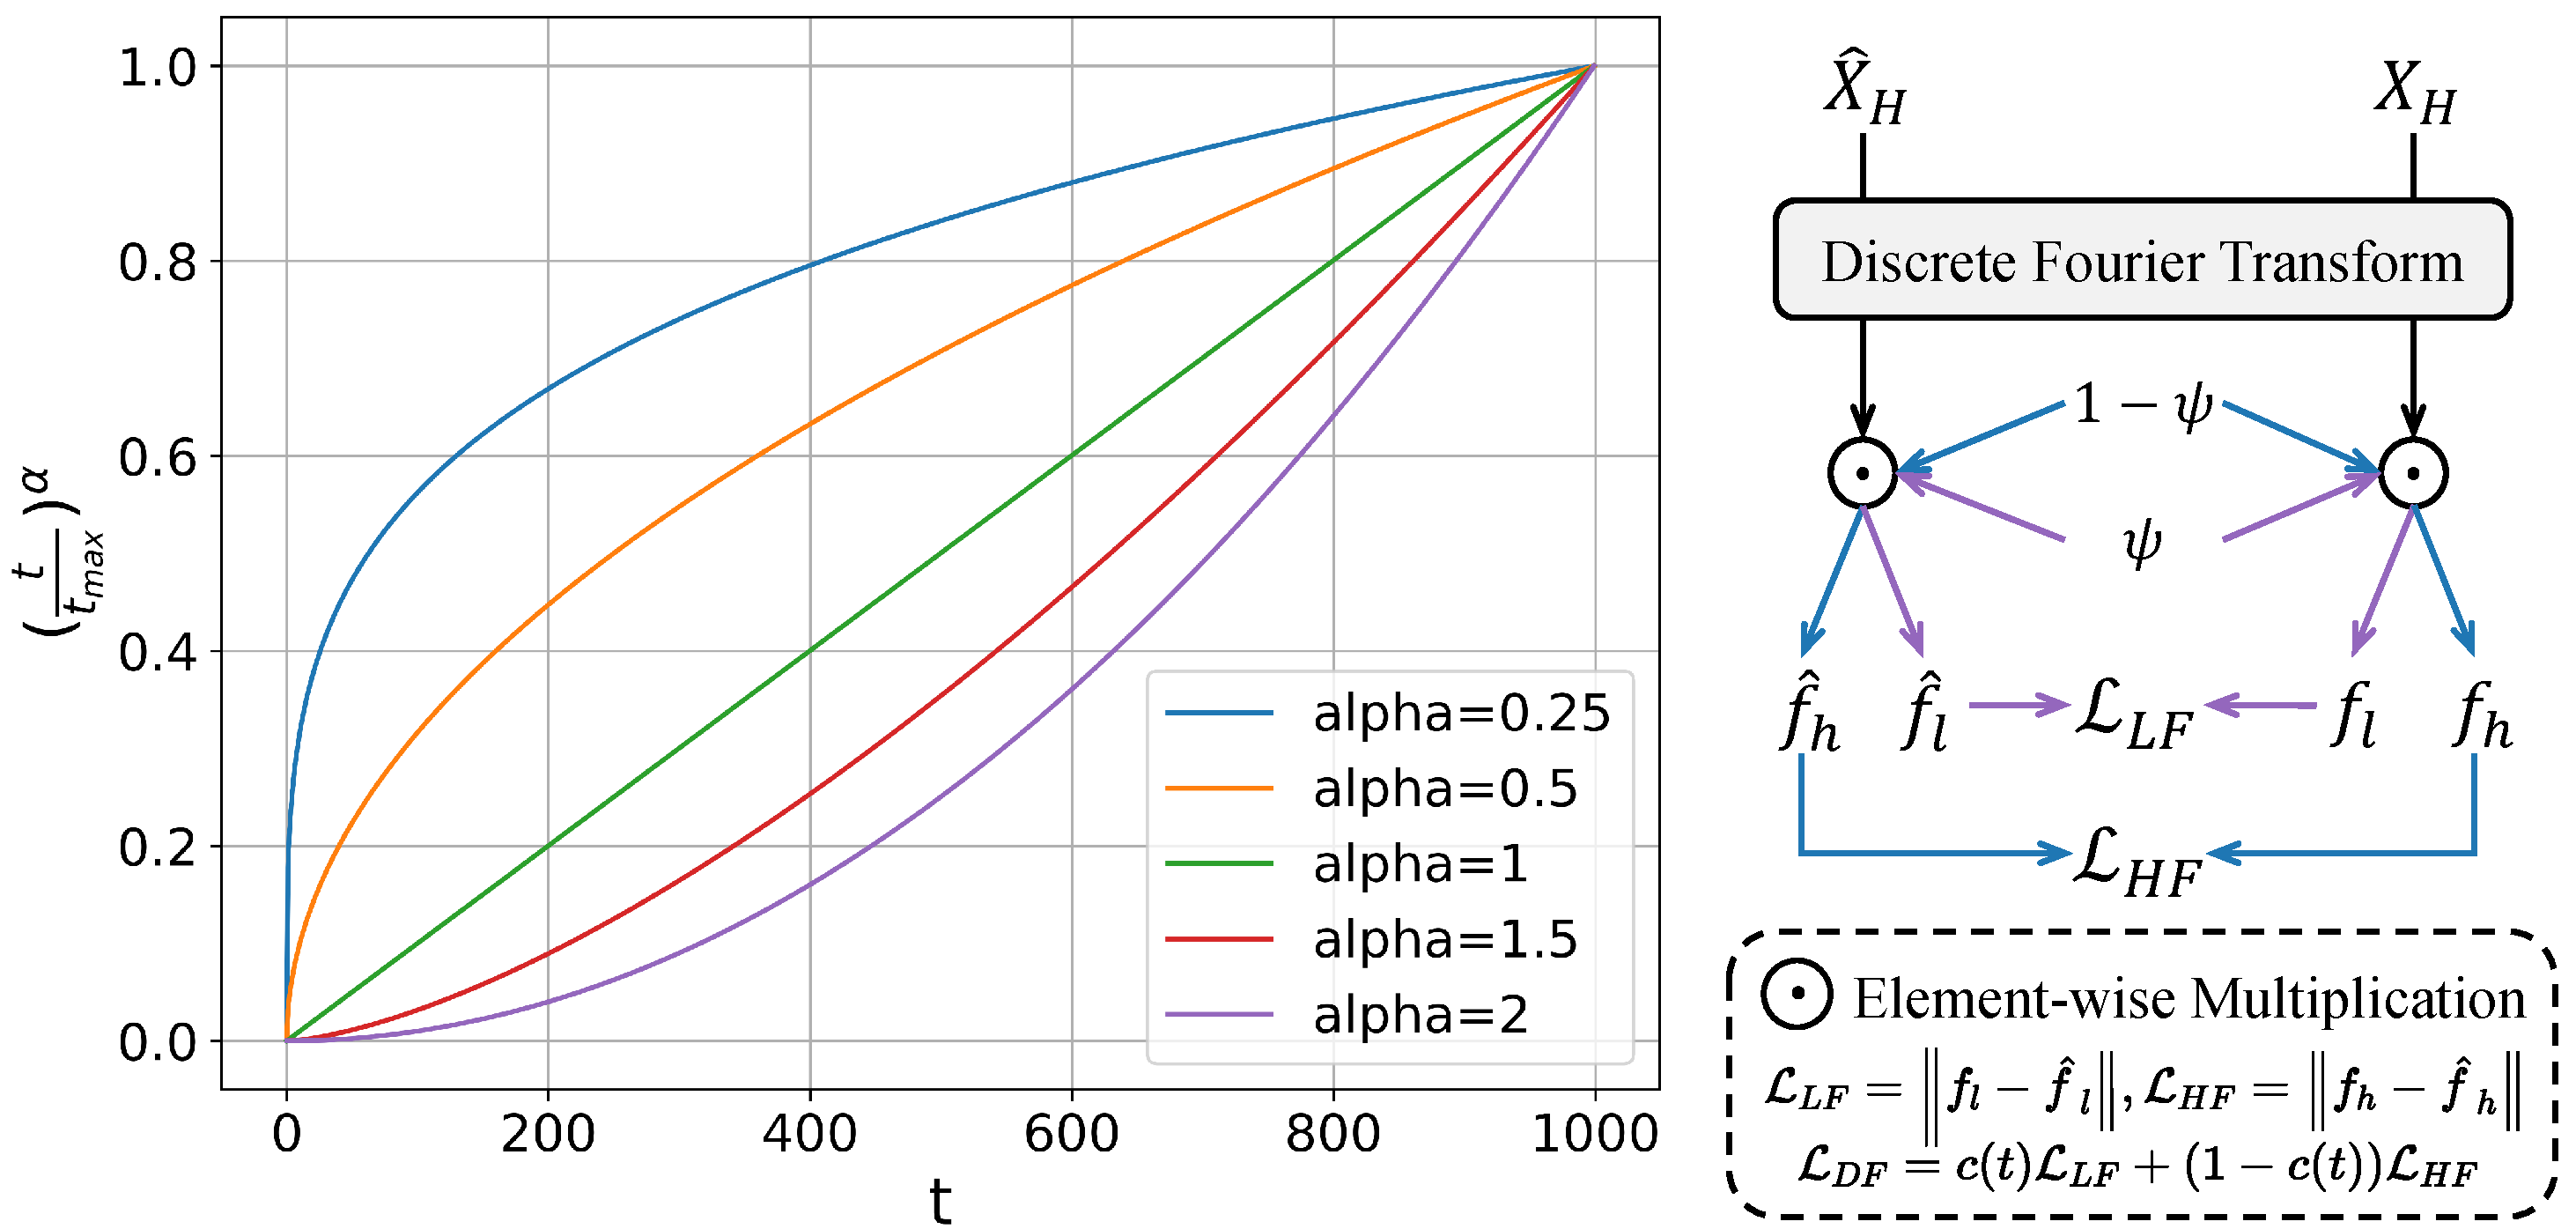
\includegraphics[width=1\linewidth]{figure/daf_method.pdf}
    \caption{\textbf{Dynamic Frequency Loss.} \textbf{Left}: curves of weighting function $c(t)$ for different $\alpha$. \textbf{Right}: details of DF loss.}
    \label{fig:daf_method}
\end{figure}

\vspace{-1em}
\paragraph{Details of DF Loss.}
% \noindent
% \textbf{Details of DF Loss.}
Here, we propose Dynamic Frequency Loss. 
Specifically, in each diffusion step $t$, we use the following equation to obtain the estimated $\hat{Z}_H$:
\begin{equation}
    \hat{Z}_H = \sigma_t^{-1}(\alpha_t\epsilon-\phi_\theta(Z_t, c_{text}, c_{l}, t)).
\end{equation}
Then, we use the decoder to convert the latent $\hat{Z}_H$ back to the pixel space, resulting in $\hat{X}_H$. After that, we apply Discrete Fourier Transform (DFT) to transform $\hat{X}_H$ into the frequency domain as shown in Figure~\ref{fig:daf_method}. 
We predefine a low-frequency pass filter $\psi$ to obtain the low- and high-frequency: %The process can be formulated below:
% Instead of using a predefined filter to separate the low- and high-frequency components, we propose a learnable adaptive filter $\psi_{\theta'}$ that takes the diffusion step $t$ and the HR video $X_H$ as inputs. The process can be formulated below:
\begin{equation}
    \hat{f}_l = \mathcal{F}(\hat{X}_H) \odot \psi, \hat{f}_h = \mathcal{F}(\hat{X}_H) \odot (1-\psi),
\end{equation}
where $\mathcal{F}(\cdot)$ is DFT, $\odot$ is element-wise multiplication. $\hat{f}_{l}$ and $\hat{f}_{h}$ denote the low and high frequency of $\hat{X}_H$. The proposed DF loss can be written as: 
\begin{equation}
    \mathcal{L}_{LF} = \| f_l - \hat{f}_l \|, \mathcal{L}_{HF} = \| f_h - \hat{f}_h \|,
\end{equation}
\begin{equation}
    \mathcal{L}_{DF} = c(t)\mathcal{L}_{LF} + (1-c(t))\mathcal{L}_{HF},
\end{equation}
where $f_l$ / $f_h$ stand for low- / high-frequency of $X_H$, respectively. $c(t) = (t/t_{max})^\alpha$ is the weighting function.